\chapter{Literature Review}
\label{chap:litreview}
\lhead{\emph{Literature Review}}

\section{Introduction}

In the dynamic and continuously evolving field of computer vision and optical character recognition (OCR), two concepts have emerged as among the significant game-changers: the Tesseract OCR engine and Convolutional Recurrent Neural Networks (CRNNs). Tesseract, initially developed by Hewlett-Packard and later adopted by Google, is a pioneering engine that converts images of text into machine-encoded text, offering groundbreaking utilities across numerous applications. On the other hand, CRNNs, a deep learning-based approach, combine the spatial feature extraction capabilities of Convolutional Neural Networks (CNNs) with the sequential data processing capacity of Recurrent Neural Networks (RNNs). These networks have set new benchmarks in the realm of scene text recognition, overcoming the challenges posed by variations in text sizes, fonts, and orientations. This literature review delves into the intricacies of these advanced tools, shedding light on their principles, applications, strengths, and potential areas for improvement, thereby enriching our understanding of current trends in OCR technology and pointing to the future possibilities.


In addition to these techniques, the selection of the correct font for each sensor is another critical element that affects the accuracy of the OCR system. Despite its importance, this aspect has been less emphasized in existing literature, thereby forming a crucial area of exploration in this study.

This literature review explores the current state of OCR technologies, with a particular focus on Tesseract and CRNN models. It delves into various image preprocessing techniques, emphasizing the unique method of red and green color masking before conversion to grayscale. Lastly, it investigates the role of font selection in enhancing OCR accuracy, thereby setting the context for the subsequent research.

While this review focuses on the promising capabilities of Tesseract OCR and Convolutional Recurrent Neural Networks (CRNNs) in the OCR domain, it's crucial to acknowledge that the OCR landscape is not limited to these technologies. Many other methods play equally significant roles in expanding the OCR frontiers and opening up new avenues for research and application. Long Short-Term Memory Networks (LSTMs), Transformers, attention-based OCR models, rule-based systems, Support Vector Machines (SVMs), Hidden Markov Models (HMMs), K-Nearest Neighbors (KNN), and template matching are some of these diverse methodologies that provide unique perspectives and solutions in the OCR realm. Each of these methods has its distinctive advantages, making them optimal for certain types of tasks, as well as its limitations, requiring continuous research and development for enhancement. However, the scope of this review will mainly revolve around Tesseract and CRNNs, while the mentioned methods provide an essential context for understanding the broader OCR ecosystem.


\section{Tesseract OCR}

\section{Convolutional Recurrent Neural Networks (CRNNs)}

\section{Other OCR Methods}

\subsection{Long Short-Term Memory Networks (LSTMs)}

Long Short-Term Memory Networks (LSTMs) are a special kind of recurrent neural network capable of learning long-term dependencies, which makes them highly suitable for OCR tasks. They've been used successfully to decode sequences of characters from images.\cite{breuelHighPerformanceOCRPrinted2013}


\subsection{Transformers}

Originally developed for natural language processing tasks, Transformer models have been adapted for OCR. They treat the OCR problem as a sequence-to-sequence translation task, translating the input image into a sequence of characters.

\subsection{Attention-based OCR models}

Attention mechanisms allow models to focus on different parts of the input image while predicting each character in the output sequence, similar to how humans read. This can improve accuracy, especially on more complex images.

\subsection{Rule-based systems}

These were some of the earliest methods for OCR and use specific rules for identifying characters based on their shape, size, and relative position. They are now less commonly used due to their limitations with complex and diverse inputs.

\subsection{Support Vector Machines (SVMs)}

Support Vector Machines (SVMs) are used for character recognition in OCR due to their effective high-dimensional mapping and classification abilities. They work best when text is clearly segmented. In the their paper, Joshua et al. used SVMs to classify characters in a license plate image and achieved an accuracy of 98.3\% using a local dataset of 10,000 images.\cite{joshuaDevelopmentImageProcessing2023}

\begin{figure}[ht]
    \centering
    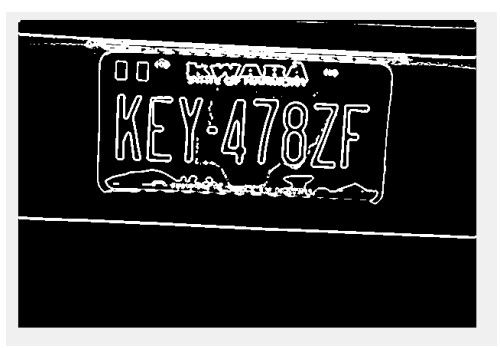
\includegraphics[width=0.6\textwidth]{Figures/SVM_Joshua.jpg}
    \caption[Development of an Image Processing Technique for Vehicle Classification using OCR and SVM]{Greyscale image with background cleaning}\cite{joshuaDevelopmentImageProcessing2023}
    \label{fig:Joshua SVM Paper}
\end{figure}





\subsection{Hidden Markov Models (HMMs)}

HMMs have been used in OCR for recognizing sequential data. HMMs are statistical models that assume an underlying process to be a Markov process with hidden states.

\subsection{K-Nearest Neighbors (KNN)}

KNN is a simple, instance-based learning algorithm used for OCR, particularly for isolated character recognition. \cite{hazraOpticalCharacterRecognition2017}

\subsection{Template Matching}

Template Matching is a technique used to locate small-parts of the bigger image which match a template image. This can be useful in OCR when the set of possible characters is known and limited.

